\flushbottom

%%
%% Expand and add a section on $\psi(z)$ and the polygamma function.
%%
%% Show that \Gamma(1-z) \Gamma(z) = \pi \csc (\pi z)
%%



%%============================================================================
%%============================================================================
\chapter{The Gamma Function}
\index{Gamma function}





%%===========================================================================
\section{Euler's Formula}
\index{Gamma function!Euler's formula}

For non-negative, integral $n$ the factorial function is
\[ n! = n(n-1) \cdots (1), \quad \mathrm{with} \quad 0! = 1. \]
We would like to extend the factorial function so it is defined for all
complex numbers.

Consider the function $\Gamma(z)$ defined by Euler's formula
\[ \Gamma(z) = \int_0^\infty\e^{-t} t^{z-1}\,\dd t.\]
(Here we take the principal value of $t^{z-1}$.)  The integral converges for
$\Re(z) > 0$.  If $\Re(z) \leq 0$ then the integrand will be at least as 
singular as $1/t$ at $t = 0$ and thus the integral will diverge.

\paragraph{Difference Equation.}
\index{Gamma function!difference equation}
Using integration by parts,
\begin{align*}
  \Gamma(z+1)
  &= \int_0^\infty\e^{-t} t^z\,\dd t \\
  &= \Big[- \e^{-t} t^z \Big]_0^\infty- \int_0^\infty- \e^{-t} z t^{z-1}\,\dd t. \\
  \intertext{Since $\Re(z) > 0$ the first term vanishes.}
  &= z \int_0^\infty\e^{-t} t^{z-1}\,\dd t \\
  &= z \Gamma(z)
\end{align*}
Thus $\Gamma(z)$ satisfies the difference equation
\[ \boxed{ \Gamma(z+1) = z \Gamma(z).} \]

For general $z$ it is not possible to express the integral in terms of 
elementary functions.  However, we can evaluate the integral for some $z$.
The value $z = 1$ looks particularly simple to do.
\[ \Gamma(1) = \int_0^\infty\e^{-t}\,\dd t = \Big[-\e^{-t}\Big]_0^\infty= 1. \]
Using the difference equation we can find the value of $\Gamma(n)$ for any 
positive, integral $n$.
\begin{align*}
  \Gamma(1) &= 1 \\
  \Gamma(2) &= 1 \\
  \Gamma(3) &= (2)(1) = 2 \\
  \Gamma(4) &= (3)(2)(1) = 6 \\
  \cdots    &= \cdots \\
  \Gamma(n+1) &= n!.
\end{align*}


Thus the Gamma function, $\Gamma(z)$, extends the factorial function to all
complex $z$ in the right half-plane.  For non-negative, integral $n$ we have
\[ \boxed{ \Gamma(n+1) = n!. } \]


\paragraph{Analyticity.}
The derivative of $\Gamma(z)$ is
\[ \Gamma'(z) = \int_0^\infty\e^{-t} t^{z-1} \log t\,\dd t.\]
Since this integral converges for $\Re(z) > 0$, $\Gamma(z)$ is analytic
in that domain.














%%============================================================================
\section{Hankel's Formula}
\index{Gamma function!Hankel's formula}

We would like to find the analytic continuation of the Gamma function into
the left half-plane.  We accomplish this with Hankel's formula
\[ \Gamma(z) = \frac{1}{\imath 2 \sin(\pi z)} \int_C \e^t t^{z-1}\,\dd t. \]
Here $C$ is the contour starting at $-\infty$ below the real axis, enclosing
the origin and returning to $-\infty$ above the real axis.  A graph of this
contour is shown in Figure~\ref{fig_hank_cont}.  Again we use the 
principle value of $t^{z-1}$ so there is a branch cut on the negative real axis.  

\begin{figure}[h!]
  \begin{center}
    %%\setlength{\unitlength}{2in}

    %%\begin{picture}(2, 1)(-1.5, -0.5)
    %%\put(0,0){\vector(1,0){0.5}}
    %%\put(0,0){\vector(-1,0){1.5}}
    %%\put(0,0){\vector(0,1){0.5}}
    %%\put(0,0){\vector(0,-1){0.5}}
    %%\thicklines
    %%\drawline(0,0)(-1.5,0)

    %%\qbezier(0.1, 0)(0.1, 0.11)(0, 0.1)
    %%\qbezier(0, 0.1)(-0.1, 0.09)(-1.5, 0.01)
    %%\qbezier(0.1, 0)(0.1, -0.11)(0, -0.1)
    %%\qbezier(0, -0.1)(-0.1, -0.09)(-1.5, -0.01)

    %%\put(0.4, 0.05){\makebox(0,0){$\Re(\xi)$}}
    %%\put(0.1, 0.45){\makebox(0,0){$\Im(\xi)$}}
    %%\end{picture}

    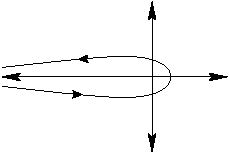
\includegraphics[width=0.3\textwidth]{ode/gamma/fig_hank_cont}
  \end{center}

  \caption{The Hankel contour.}
  \label{fig_hank_cont}
\end{figure}

The integral in Hankel's formula converges for all complex $z$.  For 
non-positive, integral $z$ the integral does not vanish.  Thus because of 
the sine term the Gamma function has simple poles at $z = 0, -1, -2, \ldots$.
For positive, integral $z$, the integrand is entire and thus the integral 
vanishes.  Using L'Hospital's rule you can show that the points, $z = 
1, 2, 3, \ldots$ are removable singularities and the Gamma function is
analytic at these points.  Since the only zeroes of $\sin(\pi z)$ occur for
integral $z$, $\Gamma(z)$ is analytic in the entire plane except for the
points, $z = 0, -1, -2, \ldots$.






\paragraph{Difference Equation.}
Using integration by parts we can derive the difference equation from
Hankel's formula.
\begin{align*}
  \Gamma(z+1)
  &= \frac{1}{\imath 2 \sin(\pi (z+1))} \int_C \e^t t^z \,\dd t \\
  &= \frac{1}{- \imath 2 \sin(\pi z)} \left( \Big[\e^t t^z\Big]_{-\infty - \imath 0}
    ^{-\infty + \imath 0} - \int_C \e^t z t^{z-1} \,\dd t \right) \\
  &= \frac{1}{\imath 2 \sin(\pi z)} z \int_C \e^t t^{z-1} \,\dd t \\
  &= z \Gamma(z).
\end{align*}

Evaluating $\Gamma(1)$,
\begin{align*}
  \Gamma(1)
  &= \lim_{z \to 1} \frac{\int_C \e^t t^{z-1}\,\dd t}{\imath 2 \sin(\pi z)}. \\
  \intertext{Both the numerator and denominator vanish.  Using L'Hospital's 
    rule,}
  &= \lim_{z \to 1} \frac{\int_C \e^t t^{z-1} \log t \,\dd t}
  {\imath 2 \pi \cos(\pi z)} \\
  &= \frac{\int_C \e^t \log t \,\dd t}{\imath 2 \pi} \\
  \intertext{Let $C_r$ be the circle of radius $r$ starting at $-\pi$ radians 
    and going to $\pi$ radians.}
  &= \frac{1}{\imath 2 \pi} \left( \int_{-\infty}^{-r}\e^t[\log(-t)-\pi i]\,\dd t
    + \int_{C_r} \e^t \log t \,\dd t
    + \int_{-r}^{-\infty} \e^t [\log (-t) + \pi i]\,\dd t \right) \\
  &= \frac{1}{\imath 2 \pi} \left( \int_{-r}^{-\infty}\e^t[-\log(-t)+\pi i]\,\dd t
    + \int_{-r}^{-\infty} \e^t [\log(-t) + \pi i] \,\dd t
    + \int_{C_r} \e^t \log t \,\dd t \right) \\
  &= \frac{1}{\imath 2 \pi} \left( \int_{-r}^{-\infty} \e^t \imath 2 \pi \,\dd t
    + \int_{C_r} \e^t \log t \,\dd t \right) \\
  \intertext{The integral on $C_r$ vanishes as $r \to 0$.}
  &= \frac{1}{\imath 2 \pi} \imath 2 \pi \int_0^{-\infty} \e^t \,\dd t \\
  &= 1.
\end{align*}
Thus we obtain the same value as with Euler's formula.  It can be shown that
Hankel's formula
is the analytic continuation of the Gamma function into the left half-plane.















%%===========================================================================
\section{Gauss' Formula}
\index{Gamma function!Gauss' formula}

Gauss defined the Gamma function as an infinite product.  This form is useful
in deriving some of its properties.  We can obtain the product form from
Euler's formula.  First recall that
\[ \e^{-t} = \lim_{n \to \infty} \left(1 - \frac{t}{n} \right)^n. \]
Substituting this into Euler's formula,
\begin{align*}
  \Gamma(z) 
  &= \int_0^\infty\e^{-t} t^{z-1}\,\dd t \\
  &= \lim_{n \to \infty} \int_0^n \left(1 - \frac{t}{n}\right)^n
  t^{z-1} \,\dd t. \\
  \intertext{With the substitution $\tau = t/n$,}
  &= \lim_{n \to \infty} \int_0^1 (1-\tau)^n n^{z-1} \tau^{z-1} n
  \,\dd \tau \\
  &= \lim_{n \to \infty} n^z \int_0^1 (1-\tau)^n \tau^{z-1}\,\dd \tau.
\end{align*}

Let $n$ be an integer.  Using integration by parts we can evaluate the integral.
\begin{align*}
  \int_0^1 (1-\tau)^n \tau^{z-1} \,\dd \tau
  &= \left[ \frac{(1-\tau)^n \tau^z}{z} \right]_0^1
  - \int_0^1 -n (1-\tau)^{n-1} \frac{\tau^z}{z} \,\dd \tau \\
  &= \frac{n}{z} \int_0^1 (1-\tau)^{n-1} \tau^z \,\dd \tau \\
  &= \frac{n(n-1)}{z(z+1)} \int_0^1 (1-\tau)^{n-2} \tau^{z+1} \,\dd \tau \\
  &= \frac{n(n-1)\cdots(1)}{z(z+1)\cdots(z+n-1)}
  \int_0^1 \tau^{z + n - 1} \,\dd \tau \\
  &= \frac{n(n-1)\cdots(1)}{z(z+1)\cdots(z+n-1)}
  \left[ \frac{\tau^{z+n}}{z+n} \right]_0^1 \\
  &= \frac{n!}{z(z+1)\cdots(z+n)}
\end{align*}

Thus we have that
\begin{align*}
  \Gamma(z)
  &= \lim_{n \to \infty} n^z \frac{n!}{z(z+1)\cdots(z+n)} \\
  &= \frac{1}{z} \lim_{n \to \infty} \frac{(1)(2)\cdots(n)}
  {(z+1)(z+2)\cdots(z+n)} n^z \\
  &= \frac{1}{z} \lim_{n \to \infty} \frac{1}{(1+z)(1+z/2)\cdots(1+z/n)}
  n^z \\
  &= \frac{1}{z} \lim_{n \to \infty} \frac{1}{(1+z)(1+z/2)\cdots(1+z/n)}
  \frac{2^z 3^z \cdots n^z}{1^z 2^z \cdots (n-1)^z} \\
  \intertext{Since $\lim_{n \to \infty} \frac{(n+1)^z}{n^z} = 1$ we can 
    multiply by that factor.}
  &= \frac{1}{z} \lim_{n \to \infty} \frac{1}{(1+z)(1+z/2)\cdots(1+z/n)}
  \frac{2^z 3^z \cdots (n+1)^z}{1^z 2^z \cdots n^z} \\
  &= \frac{1}{z} \prod_{n=1}^\infty \left[ \frac{1}{1+z/n}
    \frac{(n+1)^z}{n^z} \right] 
\end{align*}

Thus we have Gauss' formula for the Gamma function
\[ \boxed{ \Gamma(z) = \frac{1}{z} \prod_{n=1}^\infty \left[ \left(
      1 + \frac{1}{n} \right)^z \left(1 + \frac{z}{n} \right)^{-1} 
  \right]. } \]

We derived this formula from Euler's formula which is valid only in 
the left half-plane.  However, the product formula is valid for all $z$ 
except $z = 0, -1, -2, \ldots$.













%%=============================================================================
\section{Weierstrass' Formula}
\index{Gamma function!Weierstrass' formula}

\paragraph{The Euler-Mascheroni Constant.}
\index{Euler-Mascheroni constant}
Before deriving Weierstrass' product formula for the Gamma function we will
need to define the Euler-Mascheroni constant
\[ \gamma = \lim_{n \to \infty} \left[ \left(1 + \frac{1}{2} + \frac{1}{3} +
    \cdots + \frac{1}{n} \right) - \log n \right] = 0.5772\cdots. \]

In deriving the Euler product formula, we had the equation
\begin{align*}
  \Gamma(z)
  &= \lim_{n \to \infty}\left[ n^z \frac{n!}{z(z+1)\cdots(z+n)}\right]. \\
  &= \lim_{n \to \infty} \left[z^{-1} \left(1 + \frac{z}{1}\right)^{-1} 
    \left(1 + \frac{z}{2}\right)^{-1} \cdots 
    \left(1 + \frac{z}{n}\right)^{-1} n^z \right] \\
  \frac{1}{\Gamma(z)}
  &= \lim_{n \to \infty} \left[ z \left(1 + \frac{z}{1}\right)
    \left(1 + \frac{z}{2}\right)
    \cdots \left(1 + \frac{z}{n}\right) \e^{-z \log n} \right]  \\
  &= \lim_{n \to \infty} \left[ z \left(1 + \frac{z}{1}\right) \e^{-z} 
    \left(1 + \frac{z}{2}\right) \e^{-z/2} \cdots 
    \left(1 + \frac{z}{n}\right) \e^{-z/n} 
    \exp\left(\left[1 + \frac{1}{2} + \cdots + 
        \frac{1}{n} - \log n \right] z \right) \right] 
\end{align*}
Weierstrass' formula for the Gamma function is then
\[ \boxed{ \frac{1}{\Gamma(z)} = z \e^{\gamma z} \prod_{n=1}^\infty 
  \left[ \left(1+\frac{z}{n}\right) \e^{-z/n} \right]. } \]

Since the product is uniformly convergent, $1/\Gamma(z)$ is an entire function.
Since $1/\Gamma(z)$ has no singularities, we see that $\Gamma(z)$ has no 
zeros.  







\begin{Result}
  Euler's formula for the Gamma function is valid for $\Re(z) > 0$.
  \[ \Gamma(z) = \int_0^\infty \e^{-t} t^{z-1}\,\dd t \]
  Hankel's formula defines the $\Gamma(z)$ for the entire complex plane except
  for the points $z = 0, -1, -2, \ldots$.
  \[ \Gamma(z) = \frac{1}{\imath 2 \sin(\pi z)} \int_C \e^t t^{z-1}\,\dd t \]
  Gauss' and Weierstrass' product formulas are, respectively
  \[ \Gamma(z) = \frac{1}{z} \prod_{n=1}^\infty \left[ \left(1 + \frac{1}{n}
    \right)^z \left(1 + \frac{z}{n} \right)^{-1} \right]
  \qquad \mathrm{and} \]
  \[ \frac{1}{\Gamma(z)} = z \e^{\gamma z} \prod_{n=1}^\infty \left[ \left(
      1 + \frac{z}{n} \right) \e^{-z/n} \right]. \]
\end{Result}




%%=============================================================================
\section{Stirling's Approximation}
\index{Stirling's approximation}

In this section we will try to get an approximation to the Gamma function
for large positive argument.  Euler's formula is
\[ \Gamma(x) = \int_0^\infty \e^{-t} t^{x-1}\,\dd t. \]
We could first try to approximate the integral by only looking at the 
domain where the integrand is large.  In Figure~\ref{int_gamma10} the integrand
in the formula for $\Gamma(10)$, $\e^{-t} t^9$,  is plotted.  

\begin{figure}[h!]
  \begin{center}
    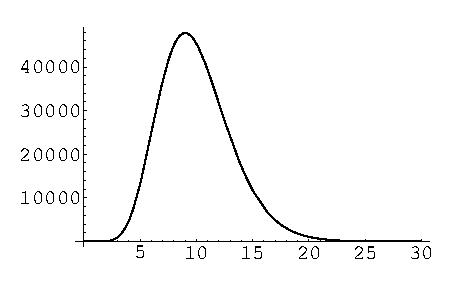
\includegraphics[width=0.4\textwidth]{ode/gamma/intgam10}
  \end{center}
  \caption{Plot of the integrand.}
  \label{int_gamma10}
\end{figure}





We see that 
the "important" part of the integrand is the hump centered around $x = 9$.
If we find where the integrand of $\Gamma(x)$ has its maximum
\begin{gather*}
  \frac{\dd}{\dd x} \left( \e^{-t} t^{x-1} \right) = 0 \\
  - \e^{-t} t^{x-1} + (x-1) \e^{-t} t^{x-2} = 0 \\
  (x-1) - t = 0 \\
  t = x-1,
\end{gather*}
we see that the maximum varies with $x$.  This could complicate our 
analysis.  To take care of this problem we introduce the change of
variables $t = x s$.  
\begin{align*}
  \Gamma(x) &= \int_0^\infty \e^{-x s} (x s)^{x-1} x\,\dd s \\
  &= x^x \int_0^\infty \e^{-x s} s^x s^{-1} \,\dd s \\
  &= x^x \int_0^\infty \e^{-x (s - \log s)} s^{-1} \,\dd s
\end{align*}
The integrands, ($\e^{-x (s-\log s)} s^{-1}$), for $\Gamma(5)$ and $\Gamma(20)$ are plotted in Figure~\ref{int_gamma520}.



\begin{figure}[h!]
  \begin{center}
    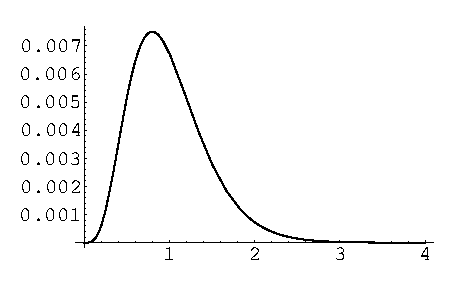
\includegraphics[width=0.4\textwidth]{ode/gamma/intgam5}
    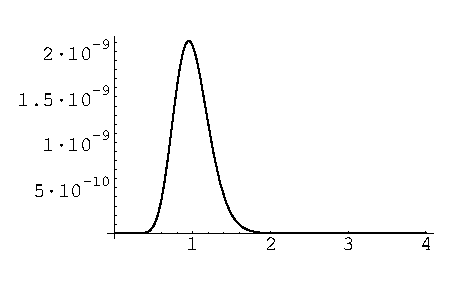
\includegraphics[width=0.4\textwidth]{ode/gamma/intgam20}
  \end{center}
  \caption{Plot of the integrands.}
  \label{int_gamma520}
\end{figure}





We see that the important part of the integrand is the hump that seems to be 
centered about $s = 1$.  Also note that the the hump becomes narrower with
increasing $x$.  This makes sense as the $\e^{-x (s - \log s)}$ term is the most
rapidly varying term.  
Instead of integrating from zero to infinity, we could get a good approximation
to the integral by just integrating over some small neighborhood centered
at $s = 1$.
Since $s - \log s$ has a minimum at $s = 1$, 
$\e^{-x (s - \log s)}$ has a maximum there.  Because the important part of the 
integrand is the small area around $s = 1$, it makes sense to approximate
$s - \log s$ with its Taylor series about that point.
\[ s - \log s = 1 + \frac{1}{2} (s - 1)^2 + O\big[(s-1)^3\big] \]
Since the hump becomes increasingly narrow with increasing $x$, we will 
approximate the $1/s$ term in the integrand with its value at $s = 1$.
Substituting these approximations into the integral, we obtain
\begin{align*}
  \Gamma(x) &\sim x^x \int_{1-\epsilon}^{1+\epsilon}
  \e^{-x (1 + (s-1)^2 / 2)}\,\dd s \\
  &= x^x \e^{-x} \int_{1-\epsilon}^{1+\epsilon}
  \e^{-x (s-1)^2/2}\,\dd s 
\end{align*}
As $x \to \infty$ both of the integrals
\[ \int_{-\infty}^{1-\epsilon} \e^{-x (s-1)^2/2}\,\dd s \qquad \mathrm{and} \qquad
\int_{1+\epsilon}^{\infty} \e^{-x (s-1)^2/2}\,\dd s \]
are exponentially small.  Thus instead of integrating from $1-\epsilon$ to
$1 + \epsilon$ we can integrate from $-\infty$ to $\infty$.
\begin{align*}
  \Gamma(x) &\sim x^x \e^{-x} \int_{-\infty}^\infty \e^{-x (s-1)^2/2}\,\dd s \\
  &= x^x \e^{-x} \int_{-\infty}^\infty \e^{-x s^2 / 2}\,\dd s \\
  &= x^x \e^{-x} \sqrt{\frac{2\pi}{x}}
\end{align*}
\[ \boxed{ \Gamma(x) \sim \sqrt{2 \pi} x^{x-1/2} \e^{-x} \quad
  \mathrm{as}\ x \to \infty. } \]

This is known as Stirling's approximation to the Gamma function.
In the table below, we see that the approximation is pretty good even for
relatively small argument.  



\[
\begin{matrix}
  n  & \Gamma(n)            & \sqrt{2 \pi} x^{x-1/2} \e^{-x} & 
  \mathrm{relative error} \\
  \hline
  5  & 24                       & 23.6038               & 0.0165 \\
  15 & 8.71783 \cdot 10^{10}       & 8.66954 \cdot 10^{10}    & 0.0055 \\
  25 & 6.20448 \cdot 10^{23}       & 6.18384 \cdot 10^{23}    & 0.0033 \\
  35 & 2.95233 \cdot 10^{38}       & 2.94531 \cdot 10^{38}    & 0.0024 \\
  45 & 2.65827 \cdot 10^{54}       & 2.65335 \cdot 10^{54}    & 0.0019
\end{matrix}
\]

In deriving Stirling's approximation to the Gamma function we did a lot of 
hand waving.  However, all of the steps can be justified and better
approximations can be obtained by using Laplace's method for finding the
asymptotic behavior of integrals.














\raggedbottom
%%============================================================================
\exercises{
\pagebreak
\flushbottom
\section{Exercises}








%%111111111111111111111111111111111111111111111111111111111111111111111111111
\begin{Exercise}
  Given that
  \[ \int_{-\infty}^\infty \e^{-x^2}\,\dd x = \sqrt{\pi}, \]
  deduce the value of $\Gamma(1/2)$.  Now find the value of $\Gamma(n+1/2)$.
\end{Exercise}




%%22222222222222222222222222222222222222222222222222222222222222222222222222222
\begin{Exercise}
  Evaluate $\int_0^\infty \e^{-x^3} \,\dd x$ in terms of the gamma function.
\end{Exercise}




%%33333333333333333333333333333333333333333333333333333333333333333333333333333
\begin{Exercise}
  Show that 
  \[
  \int_0^\infty \e^{-x} \sin( \log x ) \,\dd x = \frac{\Gamma(\imath) + \Gamma(-\imath)}{2}.
  \]
\end{Exercise}






\raggedbottom
}
%%============================================================================
\hints{
\pagebreak
\flushbottom
\section{Hints}







%%111111111111111111111111111111111111111111111111111111111111111111111111111
\begin{Hint}
  Use the change of variables, $\xi = x^2$ in the integral.  To find the
  value of $\Gamma(n+1/2)$ use the difference relation.
\end{Hint}



%%22222222222222222222222222222222222222222222222222222222222222222222222222222
\begin{Hint}
  Make the change of variable $\xi = x^3$.
\end{Hint}




%%33333333333333333333333333333333333333333333333333333333333333333333333333333
\begin{Hint}
%% CONTINUE
\end{Hint}








\raggedbottom
}
%%============================================================================
\solutions{
\pagebreak
\flushbottom
\section{Solutions}






%%111111111111111111111111111111111111111111111111111111111111111111111111111
\begin{Solution}
  \begin{gather*}
    \int_{-\infty}^\infty \e^{-x^2}\,\dd x = \sqrt{\pi} \\
    \int_0^\infty \e^{-x^2}\,\dd x = \frac{\sqrt{\pi}}{2} \\
    \intertext{Make the change of variables $\xi = x^2$.}
    \int_0^\infty \e^{-\xi} \frac{1}{2} \xi^{-1/2}\,\dd \xi = \frac{\sqrt{\pi}}{2} \\
    \boxed{ \Gamma(1/2) = \sqrt{\pi} }
  \end{gather*}
  Recall the difference relation for the Gamma function $\Gamma(z+1) = 
  z \Gamma(z)$.
  \begin{align*}
    \Gamma(n+1/2) &= (n-1/2) \Gamma(n-1/2) \\
    &= \frac{2n-1}{2} \Gamma(n-1/2) \\
    &= \frac{(2n-3)(2n-1)}{2^2} \Gamma(n-3/2) \\
    &= \frac{(1)(3)(5) \cdots (2n-1)}{2^n} \Gamma(1/2)
  \end{align*}
  \[ \boxed{ \Gamma(n+1/2) = \frac{(1)(3)(5) \cdots (2n-1)}{2^n} \sqrt{\pi} } \]
\end{Solution}







%%22222222222222222222222222222222222222222222222222222222222222222222222222222
\begin{Solution}
  We make the change of variable $\xi = x^3$, $x = \xi^{1/3}$, 
  $dx = \frac{1}{3} \xi^{-2/3} \,\dd \xi$.
  \begin{align*}
    \int_0^\infty \e^{-x^3} \,\dd x
    &= \int_0^\infty \e^{-\xi} \frac{1}{3} \xi^{-2/3} \,\dd \xi \\
    &= \frac{1}{3} \Gamma\left( \frac{1}{3} \right)
  \end{align*}
\end{Solution}





%%33333333333333333333333333333333333333333333333333333333333333333333333333333
\begin{Solution}
  \begin{align*}
    \int_0^\infty \e^{-x} \sin(\log x) \,\dd x
    &= \int_0^\infty \e^{-x} \frac{1}{\imath 2} \left( \e^{\imath \log x} - \e^{-\imath \log x}
    \right) \,\dd x \\
    &= \frac{1}{\imath 2} \int_0^\infty \e^{-x} \left( x^\imath - x^{-\imath} \right) \,\dd x \\
    &= \frac{1}{\imath 2} \left( \Gamma(1 + \imath) - \Gamma(1 - \imath) \right) \\
    &= \frac{1}{\imath 2} \left( \imath \Gamma(\imath) - (- \imath) \Gamma(- \imath) \right) \\
    &= \frac{\Gamma(\imath) + \Gamma(- \imath) }{2}
  \end{align*}
\end{Solution}







\raggedbottom
}
